\paragraph{} O processador apresenta 4 andares de \textit{pipeline} na seguinte configuração:

\begin{figure}[H]
    \centering
    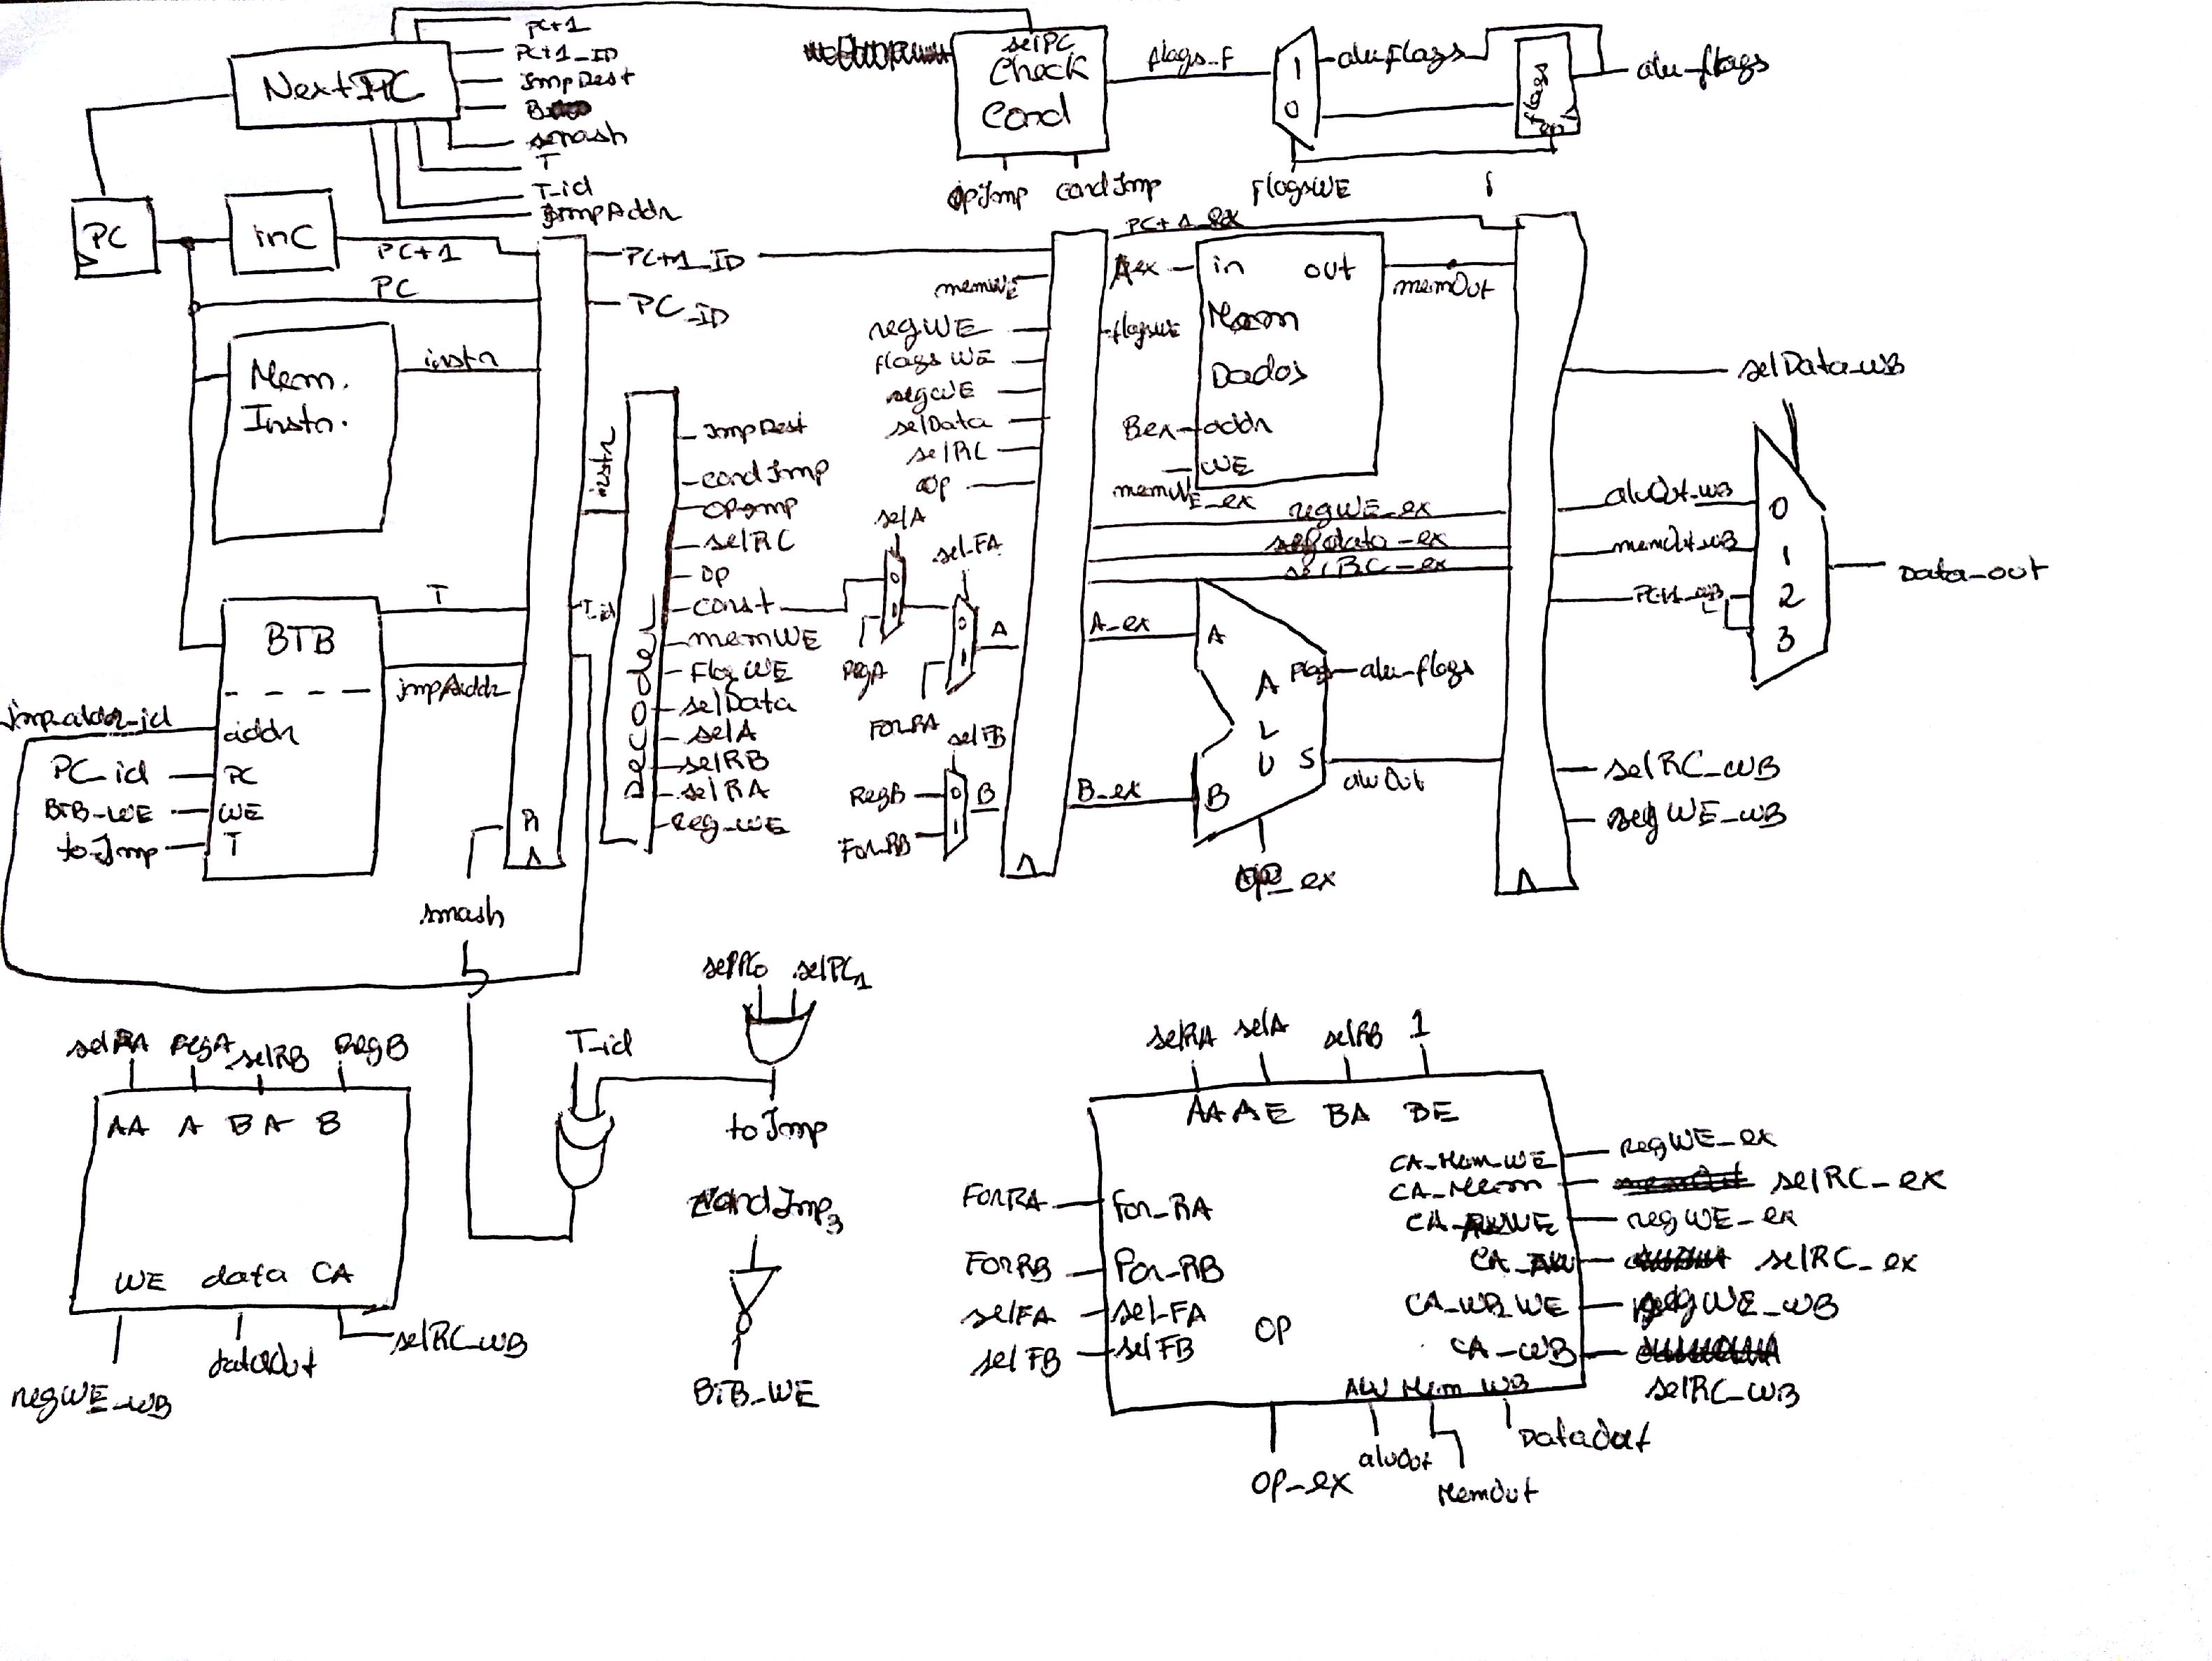
\includegraphics[width=0.8\textwidth]{./circuito.jpg}~\\[1cm]
    \caption{Circuito Geral}
    \label{fig:circuito}
\end{figure}

No primeiro andar---\textit{Instruction Fetch}---encontra-se o \textit{Branch Target Buffer}, a memória do programa, o registo do \texttt{PC} e um registo auxiliar para guardar o \texttt{PC} "original". 

No segundo andar---\textit{Instruction Decoder/Operand Fetch}---encontra-se o descodificador de instruções, os selectores dos caminhos de \textit{forwarding} e a execução do salto. O salto é executado neste andar devido a \textit{forwarding} das \textit{flags} o que resulta nos conflictos de controlo serem resolvidos com menos um \textit{stall}. A \texttt{BTB} é actualizada neste andar com a nova predição caso a instrução seja de salto.

No terceiro andar---\textit{Execute/Memory}---encontra-se a \texttt{ALU} e a memória de dados. A memória e a \texttt{ALU} não são colocados em andares diferentes pois não existem instruções de acesso à memória por endereços relativos, isto é, \texttt{R5 = M[5 + R4]}. Neste andar são usados como caminhos de \textit{forwarding} a saída da memória, a saída da \texttt{ALU} e as \textit{flags} da mesma.

No quarto andar---\textit{Write Back}---encontra-se um \textit{multiplexer} que selecciona qual a saída do 3º andar que vai ser escrita no \textit{Register File}. Também é usado o sinal de saída do \textit{multiplexer} como caminho de \textit{forwarding} para a saída do andar de \texttt{ID/OF}.

Foi introduzido um bloco para seleccionar se é preciso fazer \textit{forward} do andar de \textit{EX/MEM} ou do andar de \textit{Write Back}. Na \ref{fig:forward} apenas se indica a parte que selecciona a origem do registo A uma vez que é exactamente igual para o registo B.

\begin{figure}[H]
    \centering
    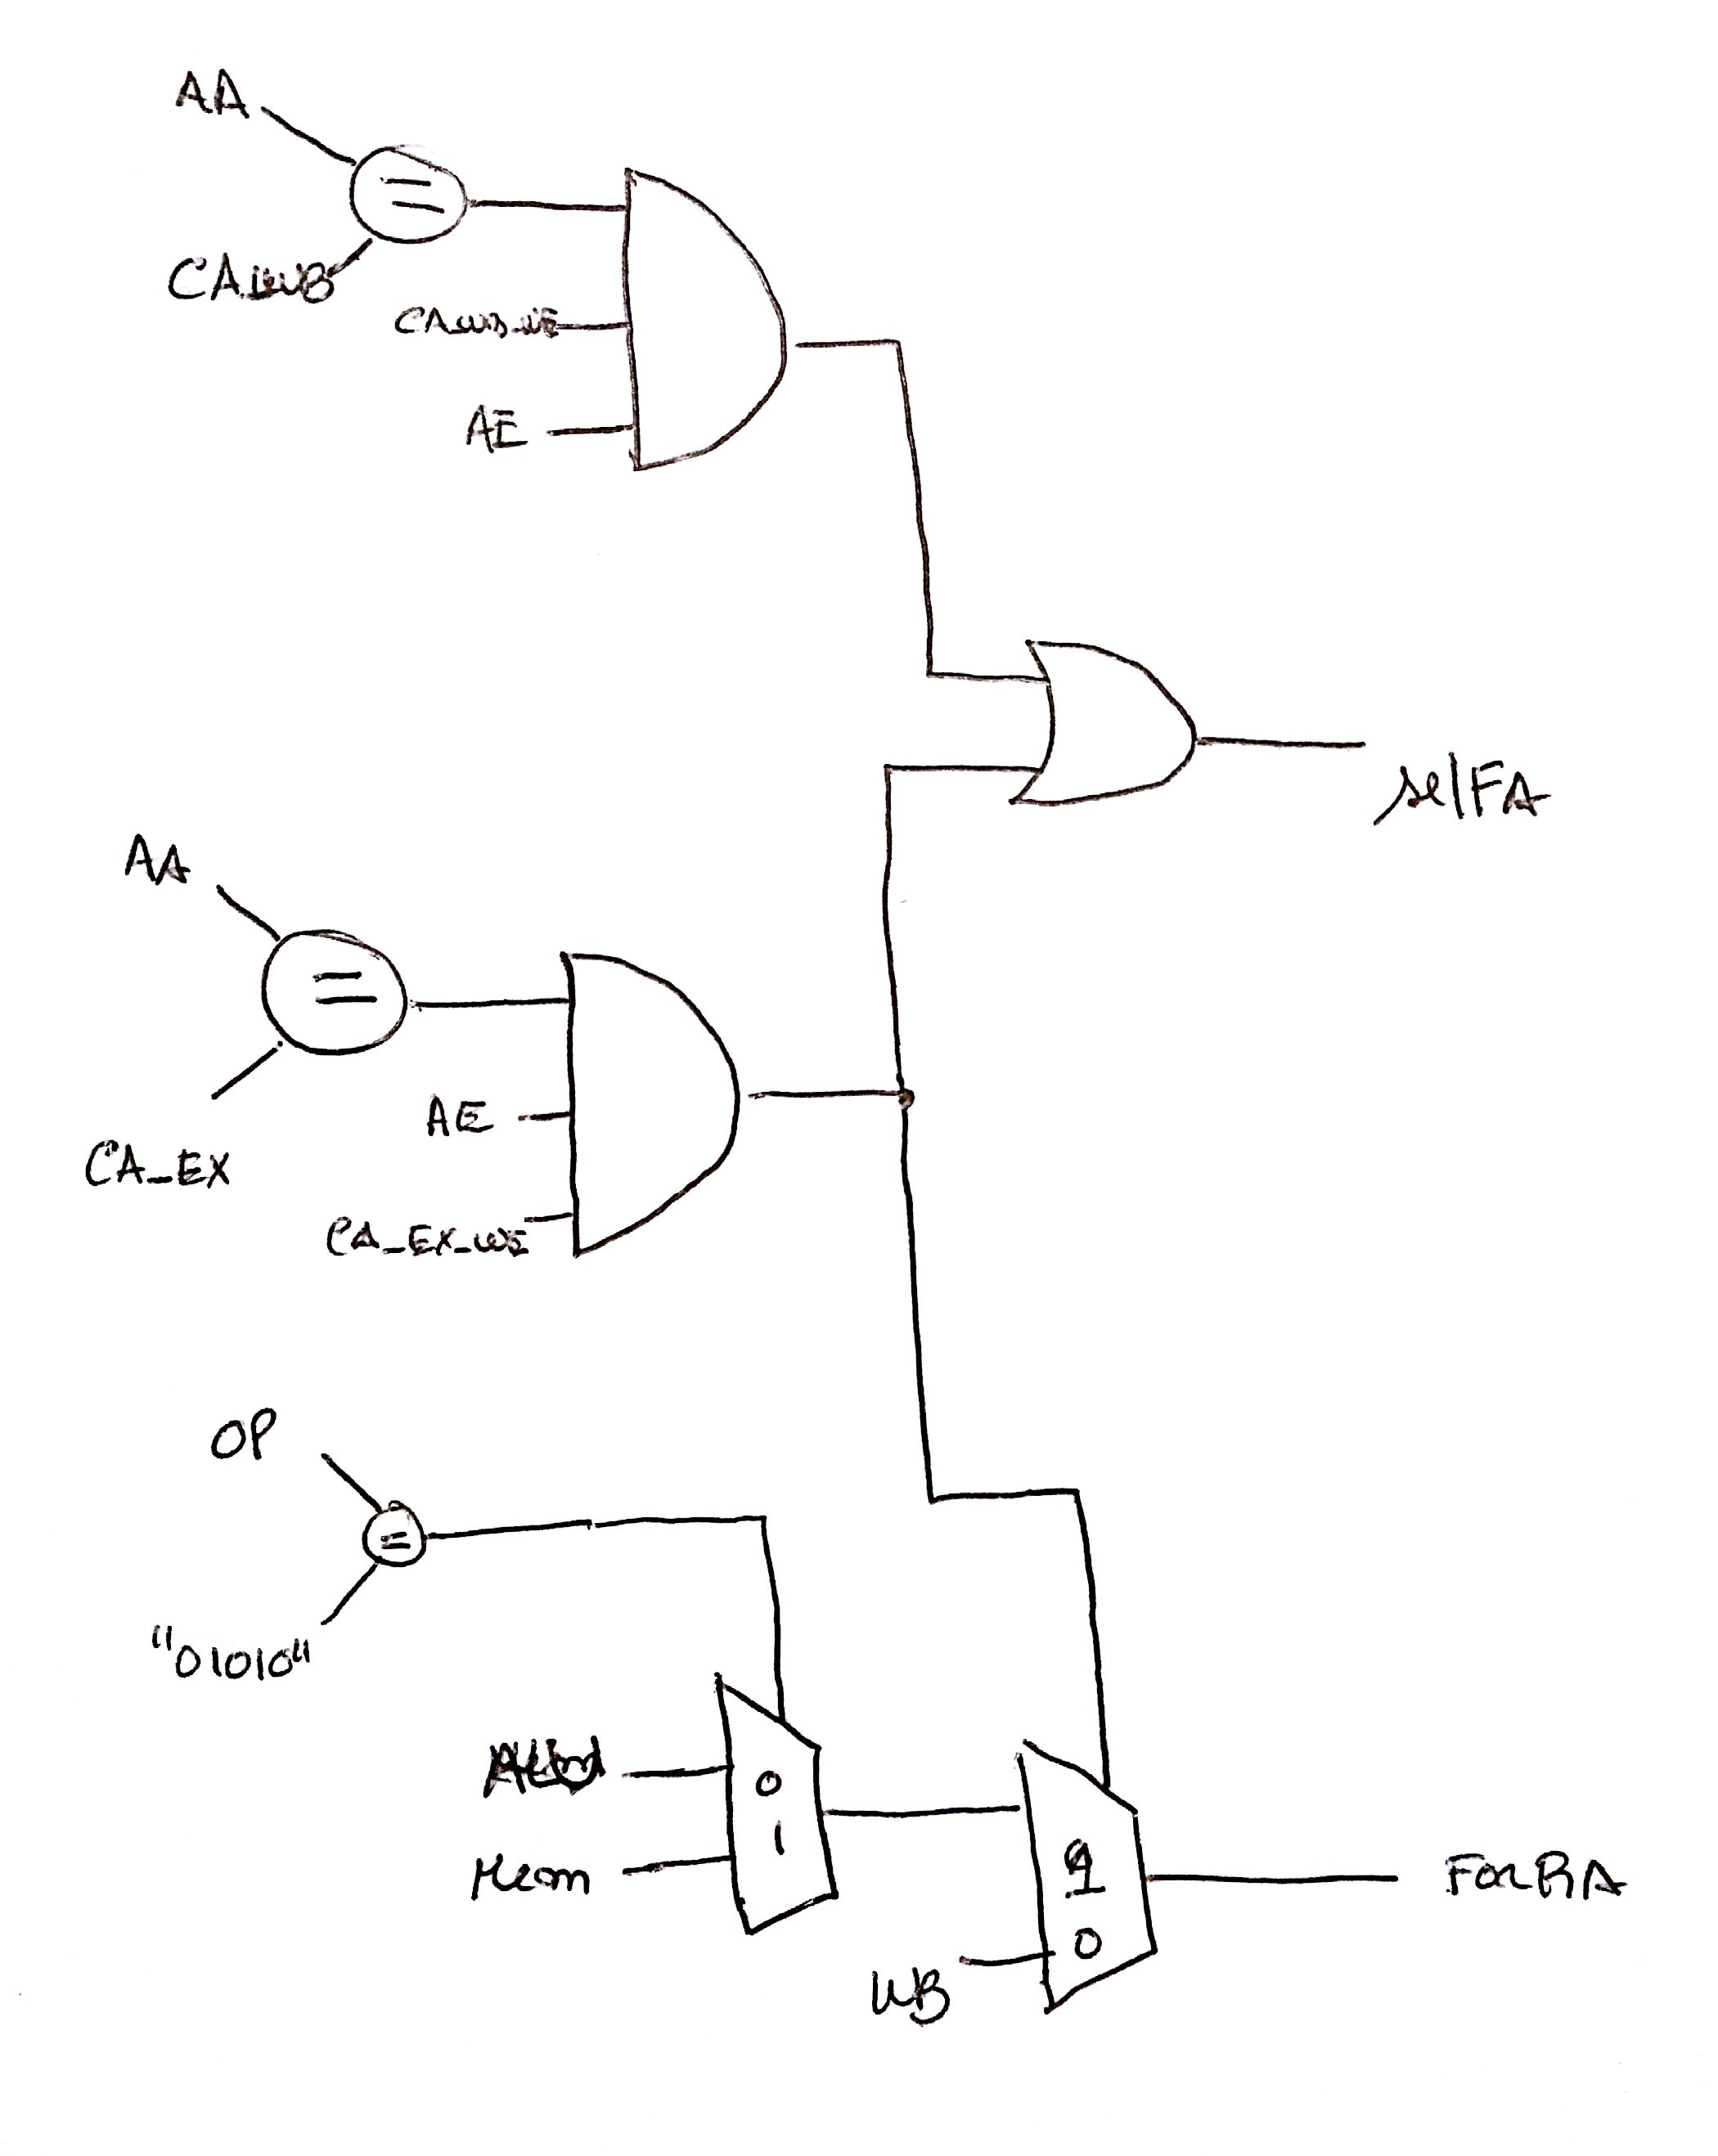
\includegraphics[keepaspectratio=true, scale=0.1]{./forward_selector.jpg}~\\[1cm]
    \caption{\textit{Forward Selector} Componente do Registo A}
    \label{fig:forward}
\end{figure}

Além deste componente foi preciso alterar a lógica que seleccionava a origem do endereço do próximo PC. O circuito utilizado é apresenta na \ref{fig:nextpc}

\begin{figure}[H]
    \centering
    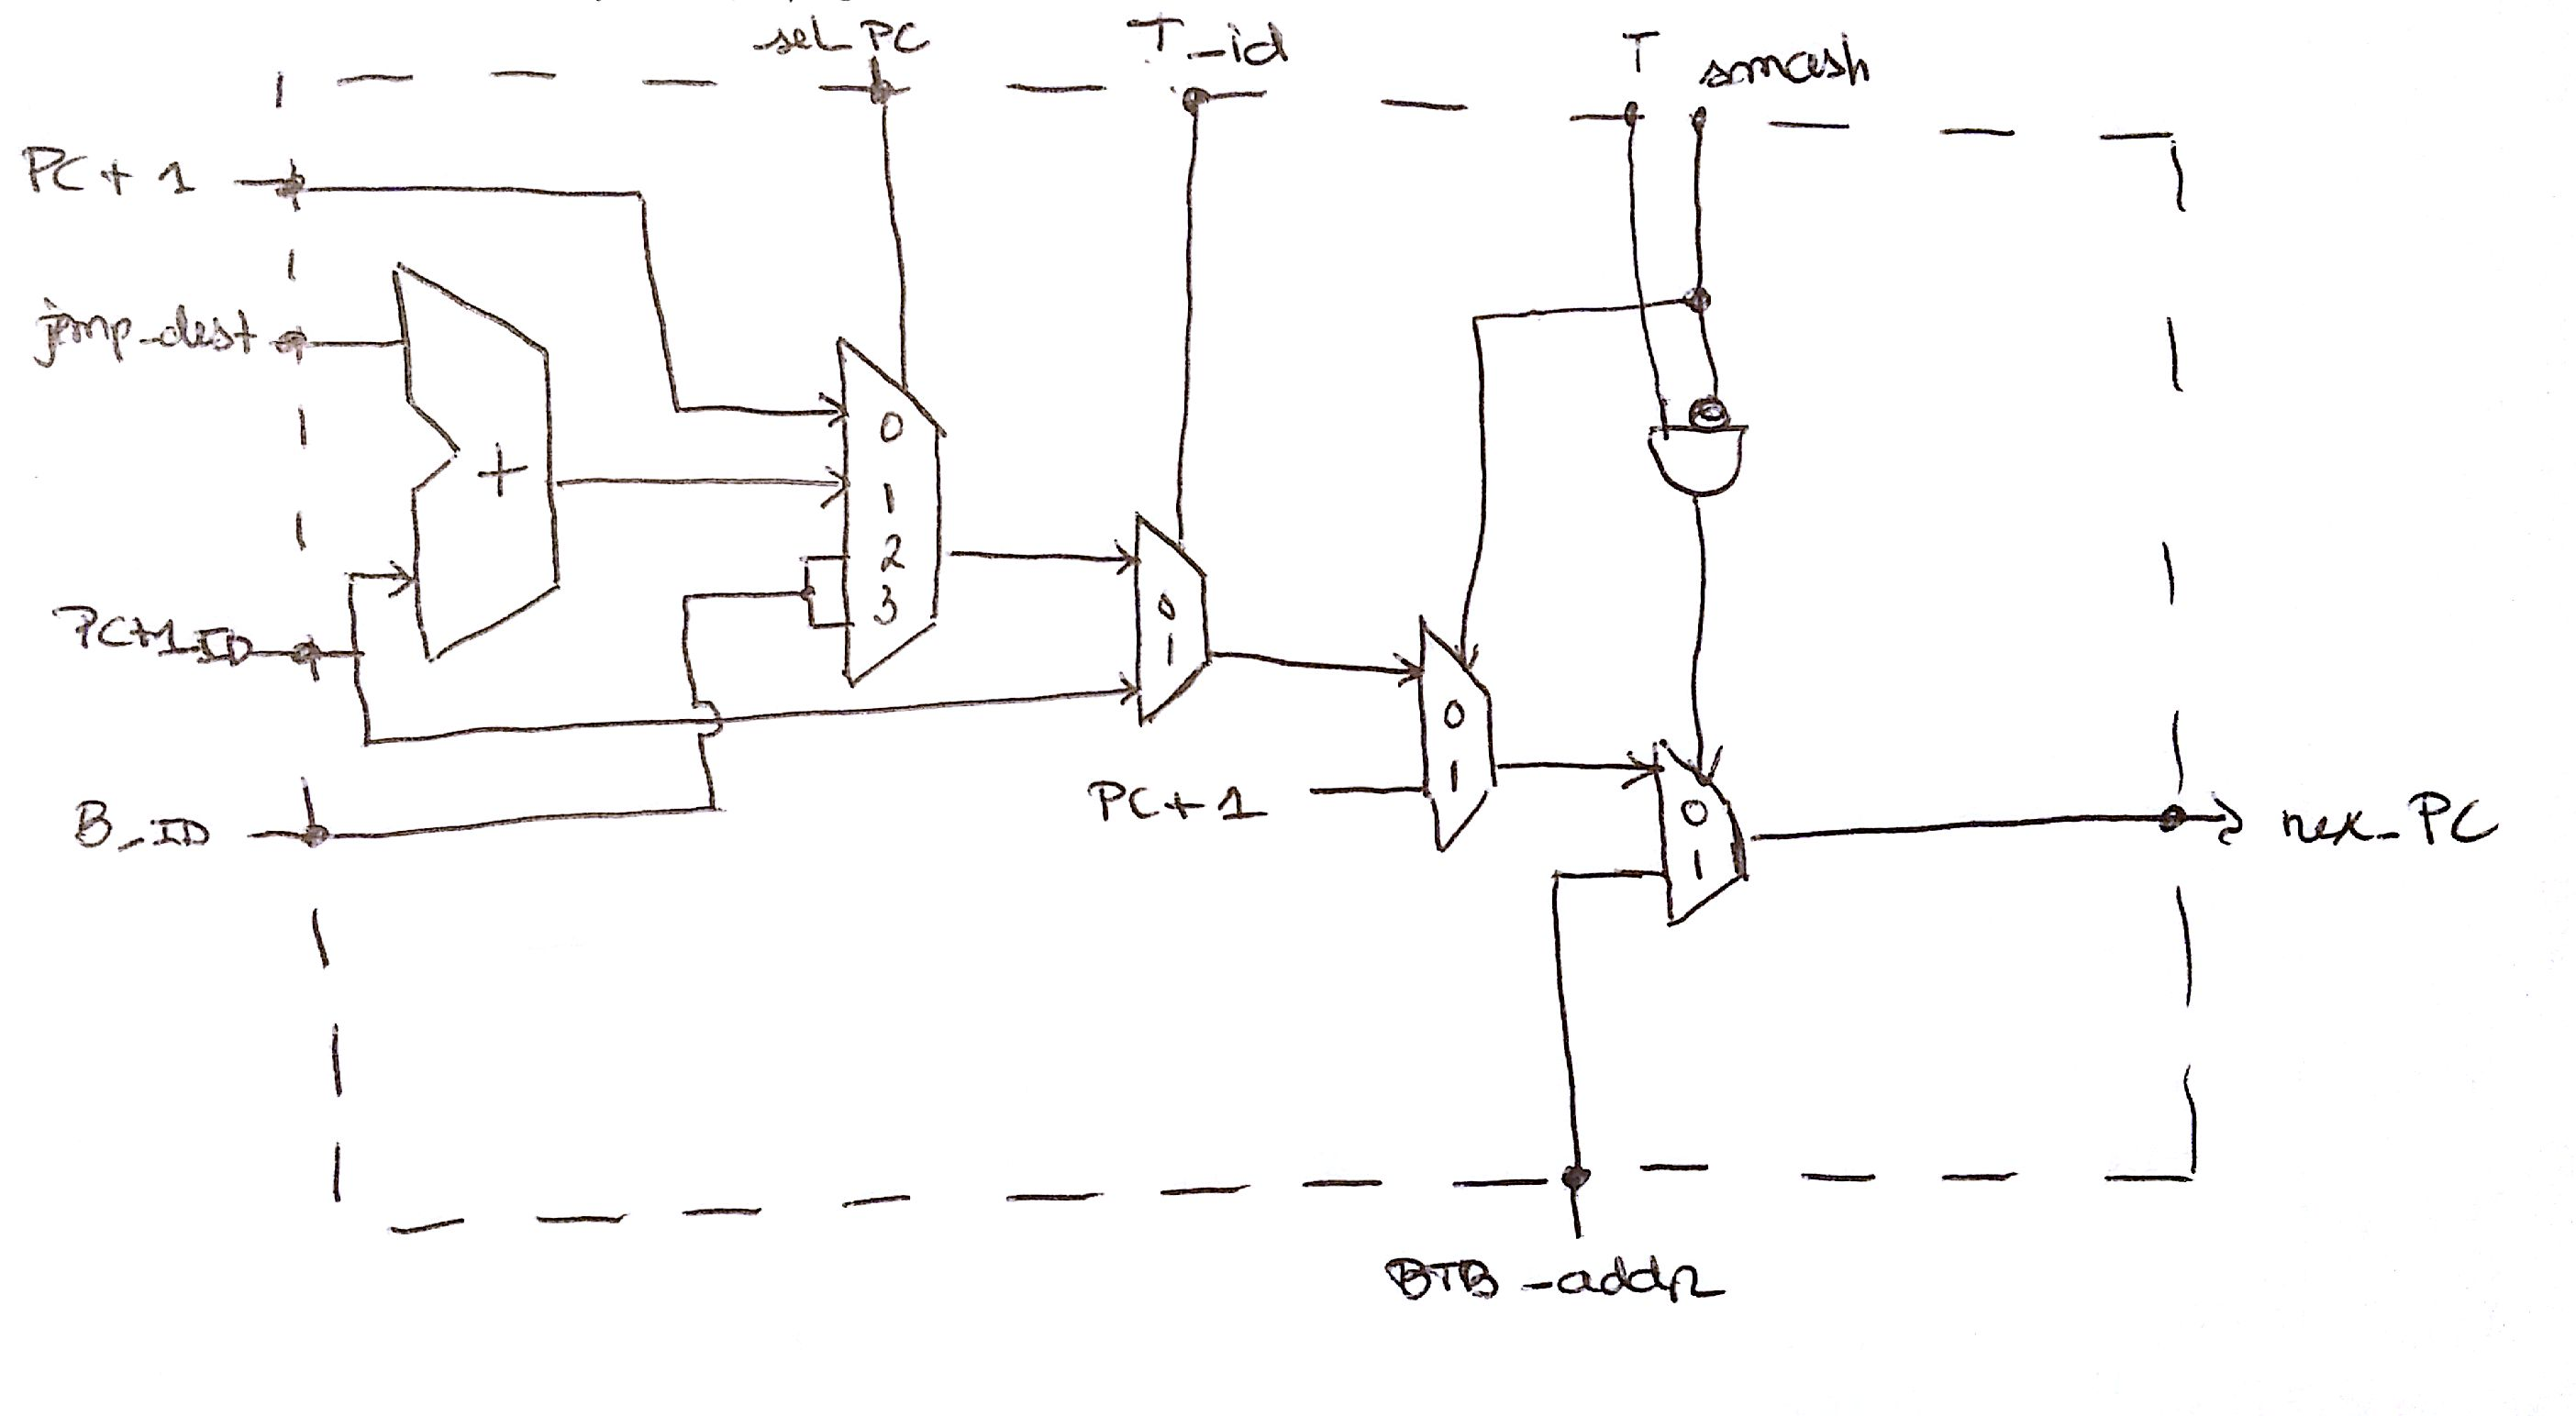
\includegraphics[width=0.8\textwidth]{./nextpc.jpg}~\\[1cm]
    \caption{Próximo PC}
    \label{fig:nextpc}
\end{figure}

